Im Rahmen dieses Praktikums soll der komplette Entwurf eines �bertragungssystems von der grundlegenden Idee bis hin zum fertigen Hardware-Konzept durchgespielt werden. Am Ende steht eine �bertragungsstrecke, die einen einfachen Bitstrom �ber einen Lautsprecher im h�rbaren Bereich �bertr�gt. Die Signale sollen �ber ein Mikrofon aufgenommen und von der nachfolgenden Schaltung demoduliert werden. Sie werden die Strecke zu gro�en Teilen mit dem Simulationstool Matlab beschreiben und simulieren. Nach erfolgreicher Simulation werden sie das beschriebene Modell in geeigneter Weise in Hardware auf einem FPGA umgesetzen, um die tats�chliche Funktion zu validieren.


%
%
%
\chapter{Konventionen}\label{sec:conventions}
%
%
%

\section{Vorbereitung}

Eine Vorbereitung auf das Praktikum w�re das Lesen des Skriptes zur Vorlesung Architekturen zur Digitalen Signalverarbeitung. Viele der darin angesprochenen Strukturen finden in diesem Praktikum Anwendung. Eine Vorbereitung selbst kann nicht stattfinden, da die verwendeten Tools einer Lizenz bed�rfen und den wenigsten somit privat zug�nglich sein werden. Gegebenenfalls ist das MATLAB-Tutorial im Anhang \ref{sec:MATLAB} lesenswert, falls man nicht schon mit MATLAB zu tun hatte oder sogar die �bung zur Vorlesung ADS besucht hat.

\section{Text}

Normaler Text, \emph{Begriffe und Fachbegriffe}, Fu�noten \footnote{Kurze weiterf�hrende Erkl�rungen oder Verweise auf selbige}

\section{Warnungen und Hinweise}

Warnungen und Hinweise werden im Skript hervorgehoben.

\prohibit{\textbf{Warnungen} werden so dargestellt. Hier kannst Du etwas kaputt machen oder Dir selbst weh tun.}

\advise{\textbf{Hinweise} werden wie hier dargestellt. Oft handelt es sich um Fallen, in die viele Neulinge treten.}

\section{Fragen und Antworten}

So sehen dann die Platzhalter f�r eure Antworten und Notizen aus:

\answergame{2}{Dies ist eine Musterl�sung}


%
%
%
\chapter{Zur Struktur}\label{sec:structure}
%
%
%

Das vorliegende Skript versucht, w�hrend des gesamten Praktikums immer neues Wissen zu vermitteln und auf altem Wissen aufzubauen. W�hrend dies in VHDL noch einfach gelingt, ist es n�tig, f�r MATLAB ein Tutorial anzuh�ngen, das vor Beginn des Praktikums durchgearbeitet werden sollte. Die einzelnen Kapitel folgen immer dem gleichen Schema, wobei oft einige der Punkte �bersprungen werden:
\begin{enumerate}
	\item Vor�berlegungen
		\begin{itemize}
			\item Idee
			\item Realisierungsm�glichkeiten finden
			\item Auswahl einer geeigneten Variante
			\item Gliederung in Teilprobleme
		\end{itemize}
	\item MATLAB
		\begin{itemize}
			\item Programmierung der Module
			\item Aufbau des Modells/der Simulation
			\item Simulation des Entwurfs
		\end{itemize}
	\item VHDL
		\begin{itemize}
			\item Verhaltensmodelle der Module entwerfen
			\item Simulation der einzelnen Module
			\item Simulation des Gesamtentwurfs
			\item Beschreibung der Hardware (RTL)
			\item Simulation des RTL Entwurfs
			\item Implementierung in Hardware
			\item Praxistest und Fehlersuche
			\item Versuchsdurchf�hrung
		\end{itemize}
\end{enumerate}

%
%
%
\chapter{Die Hardware}\label{chap:Hardware}
%
%
%

\section{Vorbereitung der Hardware}


Um �berhaupt einmal loslegen zu k�nnen, empfiehlt es sich nun, die Hardware anzuschlie�en und einzuschalten. Das SPATES\footnote{\textbf{SPATES} abk. Signal Processing And Transmission Experiments System} besitzt nur relativ wenige Anschlussm�glichkeiten (vgl. Abb. \ref{fig:ADS-Praktikum Leiterplatte} \ifthenelse{\printcolor}{gelb hinterlegt.}{grau hinterlegt.})

\begin{figure} [ht]
	\centering
		\ifthenelse{\printcolor}%
			{\includegraphics[scale=0.80]{Einf�hrung/bilder/ADS-Praktikum_Leiterplatte.eps}}%
			{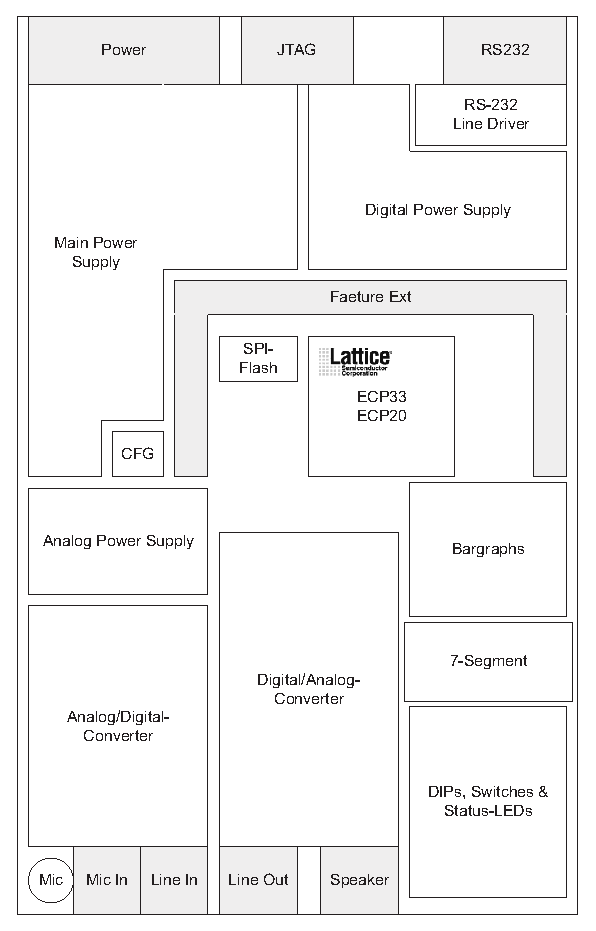
\includegraphics[scale=0.80]{Einf�hrung/bilder/ADS-Praktikum_Leiterplatte_BW.eps}}
	\caption{ADSP-SPATES}
	\label{fig:ADS-Praktikum Leiterplatte}
\end{figure}

\pargraphbox{bilder/global/esd.eps}
{
	Bei der Handhabung ist Vorsicht geboten. Es handelt sich fast ausschlie�lich um Bauteile in
	CMOS Technologie.	Zwar besitzen die Schaltkreise inzwischen sehr gute ESD-Schutzschaltungen,
	dennoch k�nnen diese durch unsachgem��e Handhabung zerst�rt werden. Da das Zeug teuer ist, 
	bitte vorher das PC-Geh�use anfassen und sich somit entladen. Dann sollte nichts passieren.
}

Zuerst schaltet Ihr das Netzger�t ein und stellt beide Spannungen auf 15V. Wieder ausmachen und eine Br�cke wie in Abb. \ref{fig:power-short} einstecken, so dass Ihr 30V Versorgungsspannung bekommt. Mit dem Adapterkabel (vgl. Abb. \ref{fig:power-cable}) verbindet Ihr das Netzger�t mit dem SPATES. Der Stecker geht manchmal etwas schwerer, allerdings sollte man keine Gewalt oder ein Messer anwenden m�ssen.


\begin{figure}[ht]
	\centering
	\begin{minipage}[b]{.4\linewidth}
		\centering
		\includegraphics[height=20ex]{Einf�hrung/bilder/power_short.eps}
		\caption{Die Netzteil-Br�cke}
		\label{fig:power-short}
	\end{minipage}
	\begin{minipage}[b]{.4\linewidth}
	  \centering
		\includegraphics[height=10ex]{Einf�hrung/bilder/power_cable.eps}
		\caption{Power cable}
		\label{fig:power-cable}
	\end{minipage}
\end{figure}

Anschlie�end k�nnt Ihr das Netzteil wieder einschalten. Zuerst sollten euch die verschiedenen Versorgungsspannungs-LEDs auffallen, die eine Funktion der einzelnen Spannungsebenen signalisieren (oder eben auch nicht). Nach einem kurzen Bootvorgang, der durch 2 LEDs direkt neben dem FPGA signalisiert wird, startet auch schon das Diagnose-Programm. Hierbei werden alle LEDs, die 7-Segment-Anzeigen und die Bargraphs kurz angesteuert. Falls Ihr den Lautsprecher schon angeschlossen habt, m�sste danach ein kurzer Sweep\footnote{Durchfahren eines Frequenzbereichs z.B. 20Hz bis 20kHz} zu h�ren sein. Ist dieser Test abgeschlossen, so kann man interaktiv alle weiteren Bedienelemente testen. Dabei gilt die Zuordnung aus Tabelle \ref{tab:s2led-assignment}.

\begin{table}[ht]
	\centering
	\begin{tabular}{|c|c|}\hline
		\textbf{Schalter/Taster} & \textbf{Anzeigeelement}\\\hline
		S1 & Alle Segmente LD1 \\\hline
		S2 & Alle Segmente LD2 \\\hline
		S3 & Alle Segmente LD3 \\\hline
		S4 & Alle Segmente LD4 \\\hline
		S5 & Alle Segmente Bargraph 1,2 \\\hline
		S6 & Status 1R, 1Y, 1G \\\hline
		S7 & Status 2R, 2Y, 2G \\\hline
		S8 & Status 3R, 3Y, 3G \\\hline
		DIP 1-8 & Bargraph 1,2 LEDs 1-8 \\\hline
	\end{tabular}
	\caption{Zuordnungen der Taster und Schalter}
	\label{tab:s2led-assignment}
\end{table}